% Editable intermediate poster; compiles from paper/ using the original manuscript figures.
% Requires: paper/generated/confirmation_effects.pdf and discovery_allocation.pdf
\documentclass{article}
\usepackage[paperwidth=841mm,paperheight=1189mm,margin=32mm]{geometry}
\usepackage[T1]{fontenc}
\usepackage{graphicx,amsmath,amssymb,booktabs,array}
\usepackage[hidelinks]{hyperref}
\pagestyle{empty}
\setlength{\parindent}{0pt}
\setlength{\parskip}{5mm}
\newcommand{\heading}[1]{\par\vspace{15mm}{\fontsize{34}{40}\selectfont\bfseries #1}\par\vspace{2mm}\hrule height 1pt\vspace{5mm}}
\newcommand{\bodyfont}{\fontsize{28}{38}\selectfont}
\newcommand{\note}[1]{{\fontsize{22}{31}\selectfont #1}}
\begin{document}
{\fontsize{20}{26}\selectfont NEURIPS 2026 / ROBOPAD \hfill MACHINE INTELLIGENCE SUMMIT / Z\"URICH}\par
\vspace{9mm}
{\fontsize{72}{79}\selectfont\bfseries Refinement versus Refresh}\par
\vspace{4mm}
{\fontsize{35}{43}\selectfont Compute Allocation for Closed-Loop Robot Policies}\par
\vspace{7mm}
{\fontsize{23}{30}\selectfont Alba Mar\'ia T\'ellez Fern\'andez \quad MAAT Institute}\par
\vspace{7mm}\hrule height 2pt\vspace{9mm}
{\fontsize{41}{49}\selectfont\bfseries Why did fewer denoising steps improve closed-loop success?}\par
\vspace{6mm}
{\fontsize{26}{35}\selectfont At a fixed two-action replanning prefix, reducing denoising from five steps to two improves success from \textbf{122/160 to 139/160}. The experiment changes the solver budget without changing the frozen policy checkpoint.}\par
\vspace{9mm}
\begin{minipage}[t]{.48\linewidth}
\heading{01 / The actual control trade-off}
\bodyfont
A chunked VLA generates a future action sequence from observation $o_t$. The robot executes $h$ actions before obtaining $o_{t+h}$ and generating a new chunk. Increasing denoising depth $d$ spends more compute refining the current prediction; reducing $h$ spends compute on fresher feedback.
\[
\boxed{b(h,d)=\frac{F_{\mathrm{gen}}(d)}{h}}\qquad
\boxed{C_e=\left\lceil\frac{T_e}{h}\right\rceil F_{\mathrm{gen}}(d)}
\]
\note{The first quantity is nominal arithmetic per control step; the second counts every generated chunk per episode, including partly consumed final chunks. Neither is physical-robot latency.}
\heading{02 / Paired primary result}
{\fontsize{64}{72}\selectfont\bfseries +10.6 pp}\par
\vspace{2mm}
\bodyfont 139/160 at $(h,d)=(2,2)$ versus 122/160 at $(2,5)$; 24 paired wins, seven losses, and 129 ties.\par
\note{Descriptive task-conditional 95\% interval: +4.4 to +16.9 percentage points. State bootstrap within eight fixed tasks, retaining paired seeds.}
\heading{03 / Why the savings are limited}
{\fontsize{61}{70}\selectfont\bfseries 82.1\%}\par
\bodyfont of native generation arithmetic is denoising-independent. Reducing $d$ from five to two at $h=2$ reduces reference-calibrated neural arithmetic per control step by only \textbf{5.9\%}.
\heading{04 / Evaluation split}
\bodyfont
\textbf{Discovery:} 12 configurations, four Spatial tasks, 480 attempts.\par
\textbf{Confirmation:} seven frozen settings, eight separate Goal/Object tasks, 1,120 attempts. The primary contrast was frozen before the task-transfer evaluation.
\end{minipage}\hfill
\begin{minipage}[t]{.48\linewidth}
\heading{05 / Original confirmation figure}
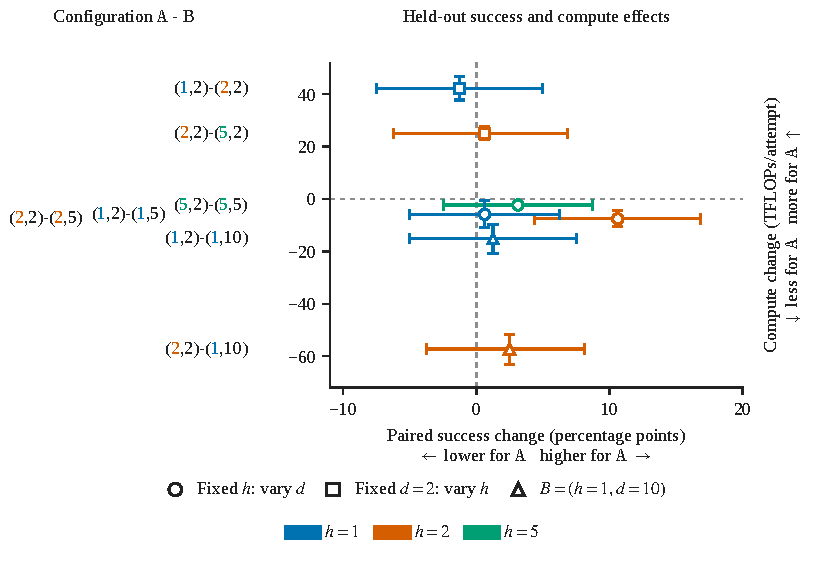
\includegraphics[width=\linewidth]{generated/confirmation_effects.pdf}\par
\note{\textbf{Reused from the accepted manuscript, Figure 2.} Filled diamond: prespecified fixed-prefix primary contrast. Other frozen denoising contrasts and later-amended descriptive contrasts are distinguished; secondary intervals are unadjusted.}
\heading{06 / Original discovery figure}
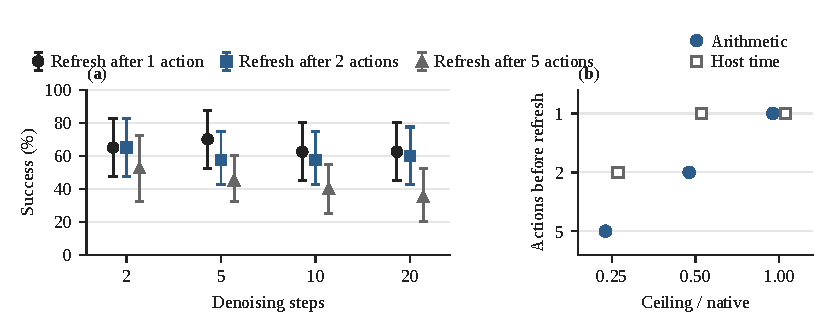
\includegraphics[width=\linewidth]{generated/discovery_allocation.pdf}\par
\note{\textbf{Reused from the accepted manuscript, Figure 1.} Discovery success across denoising counts and prefixes (left), and sensitivity of feasible prefix selection to arithmetic versus host-time constraints (right).}
\heading{07 / Refresh has a different effect}
\bodyfont
At $d=2$, increasing the executed prefix from $h=2$ to $h=5$ yields \textbf{139/160 versus 138/160} observed successes, while reducing reference-calibrated episode arithmetic from 41.1 to 16.1 TFLOPs (\textbf{60.7\%}). Equivalent quality is \emph{not} established.
\heading{08 / Interpretation, not an optimal scheduler}
\bodyfont
The evidence shows non-monotonic closed-loop success under additional denoising for this checkpoint and task population. The cause is not identified. Changing $h$ also changes the positions of the predicted actions that are executed, not only observation freshness. No universal optimal allocation, asynchronous speedup, or real-robot transfer is established.
\end{minipage}
\vfill
\hrule height 1.5pt\vspace{6mm}
{\fontsize{19}{26}\selectfont \textbf{Work in progress poster} \quad Original manuscript figures, grayscale for print. \hfill \url{github.com/amtellezfernandez/refinement-refresh-robot-policies}}\par
\end{document}
